\chapter{Projekt i implementacja}

\section{Wykorzystane technologie}
\subsection{Python 3.8.1}
Do implementacji algorytmu został użyty Python. Jest to najpopularniejszy język programowania w domenie uczenia maszynowego. Wymagana jest wersja 3.8 lub wyższa ze względu na użycie w implementacji metod dostępnych od tej wersji.  
\subsection{PonyGE2}
PonyGE2 \cite{Fenton_2017} jest implementacją ewolucji genetycznej w języku Python. Pozwala na łatwą konfigurację parametrów ewolucji genetycznej oraz możliwość dodania własnych problemów, a także sposobów ewaluacji rozwiązań. Niestety, PonyGE2 nie jest przystosowane do bycia dołączaną jako niezależna biblioteka i nie umożliwia dostępu poprzez wygodny interfejs.

\begin{figure}[h]
	\centering{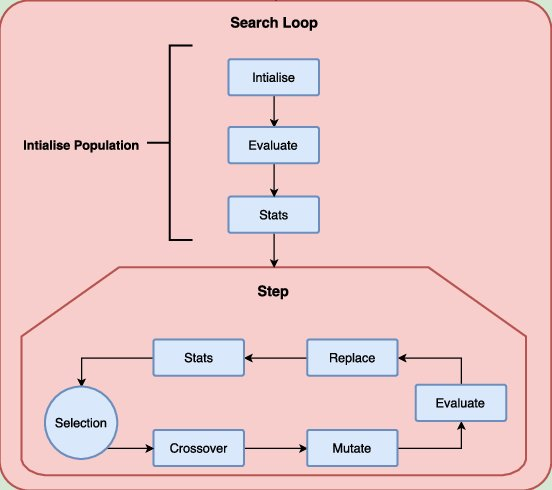
\includegraphics{PonyGE2-search-loop.jpg}}
	\caption{\label{fig:PonyGE2-search-loop}Ogólny schemat działania PonyGE2}
\end{figure}

\section{Tworzenie gramatyki procesu biznesowego}
\label{sec:businessGrammarCreation}
Projektując gramatykę procesu biznesowego, przyjęto dwa początkowe założenia. Uznano, że generowane modele muszą być łatwe do przełożenia na notację BPMN oraz nie powinny być tworzone modele niespójne strukturalnie, co pozwali na zredukowanie przestrzeni rozwiązań, jednocześnie gwarantując tworzenie niegenerujących błędów modeli.

Przy tworzeniu gramatyki procesu biznesowego ważne jest, żeby znaleźć balans, jeśli chodzi o poziom skomplikowania modelu, jaki będzie możliwy do wygenerowania, używając zaproponowanej gramatyki.  W pracy \cite{10.1007/978-3-540-69534-9_35} przeanalizowano składniki języka BPMN pod kątem częstotliwości ich stosowania. Najczęściej używanymi elementami modelów procesu biznesowego, jeśli chodzi o bramki, są: XOR - ALBO kodowane w proponowanej gramatyce jako xor, AND - I jako and oraz pętle jako lo<0$\_$n>. Do przedstawionej dalej gramatyki dodano także bramki OR - LUB reprezentowane jako opt. Ponadto konieczne jest użycie symbolu seq, która oznacza, że aktywności następują kolejno po sobie.

Zgodnie z zaleceniami w sekcji \ref{sec:modelling} przyjmuje się, że dobrą praktyką jest, żeby model zawierał tylko jedno zdarzenie początkowe i końcowe. Z tego powodu przyjęto, że zdarzenia te są domyślnie odpowiednio na początku i końcu wygenerowanego słowa i nie są one jawnie reprezentowane w gramatyce.

W sekcji \ref{grammarCreation} opisano problemem ewolucji gramatyki dla metod opartych o krzyżowanie i mutację punktową lub n-punktową, dlatego zdecydowano się na stworzenie gramatyki pod kątem wersji tych operatorów używających fenotypu - drzewa. Lokalne przeszukiwanie często staje się słabym punktem algorytmów ewolucyjnych. Stosując wspomniane operatory, prawdopodobna jest sytuacja, że mała modyfikacja blisko korzenia może poprawić rozwiązanie, jednak jej zaistnienie wymaga wygenerowania identycznego poddrzewa na nowo, przez co prawdopodobieństwo zaistnienia takiej sytuacji jest niskie. Do rozwiązania tego problemu mogą służyć metody inspirowane algorytmami memetycznymi, a  działające na drzewach \cite{memetic}. Dają one możliwość aplikowania lokalnych zmian bez konieczności powtórnego generowania całego poddrzewa, co pozwala na usprawnienie procesu ewolucji. Niestety, użyta biblioteka nie posiada podobnych metod lokalnej optymalizacji. Żeby w pewnym stopniu zaradzić temu problemowi, zmniejszono głębokość potrzebnego do reprezentacji modelu drzewa, jednocześnie zwiększać szanse na lokalne mutacje poprzez wprowadzenie symbolu nieterminalnego <slots>. Sprawia to, że drzewo rośnie bardziej wszerz i oprócz jednego symbolu <anygate>, którego użycie ma zapewnić tworzenie poprawnych, niepustych rozwiązań, generowane są symbole <slot>, które mogą pozostać puste lub wygenerować symbol <anygate> z 10\% prawdopodobieństwem. Przekłada się to na większą ilość lokalnych zmian na późniejszych etapach ewolucji. Lokalne przeszukiwania wspomaga także poprzez reprezentowanie bramki jako dwa odrębne symbole - <name>(<slots>). Dzięki temu w wyprowadzeniu nazwa bramki <name> jest oddzielona on jej zawartości, co sprawia, że możliwa jest zmiana nazwy bramki bez modyfikacji jej wnętrza.

Zaadresowano również konieczność odwzorowania w gramatyce częstotliwości występowania poszczególnych bramek logicznych. Zgodnie z \cite{10.1007/978-3-540-69534-9_35} połączenia i bramki XOR - ALBO, AND - I są tworzone przez większą ilość produkcji niż rzadziej występujące pętle i bramki OR - LUB. 

Zapis GE{\_}RANGE:n jest rozszerzeniem notacji zapewnianym przez PonyGE2, które umożliwia dodanie wygodne dodanie n zmiennych, czyli GE{\_}RANGE:2 w BNF oznacza 0|1|2.
Podobny jest zapis GE{\_}RANGE:dataset{\_}vars, który umożliwia dodanie ilości zmiennych odpowiadającej ich ilości w zbiorze danych w tym wypadku w liczbie aktywności w dzienniku zdarzeń. Został on dodany, dzięki rozszerzeniu standardowego, zapewnianego przez PonyGE2 parsera gramatyki.

Wszystkie bramki mają nazwy tej samej długości - 3 znaki, co ułatwia parsowanie gramatyki. Symbol startowy to <e>.

\begin{figure}[!ht]
\lstset{caption=Proponowana gramatyka procesu biznesowego, captionpos=b}
\lstset{label=src:grammar, frame=single}
\begin{lstlisting}
<e> ::= <slot><slot><anygate><slot><slot>

<anygate> ::=  <anygate><anygate> | <name>(<slots>) | {<event>}

<slot> ::= <anygate> | '' | '' | '' | '' | '' | '' | '' | '' | ''

<slots> ::= <slot><slot><anygate><slot><slot>

<name> ::= and | xor | seq | and | xor | seq | and | xor | seq | 
           and | xor | seq | and | xor | seq | lo<0_n> | lo<0_n> |opt

<event> ::= GE_RANGE:dataset_vars

<0_n> ::= GE_RANGE:5
\end{lstlisting}
\end{figure}

Model, dla którego zaprezentowanie obliczanie metryk (rys. \ref{fig:metrics_business_process}) byłby za pomocą powyższej notacji zakodowany jako:
\begin{center}
(\{a\}and(\{b\}\{c\})opt(\{b\}\{e\})\{d\}
\end{center}

Zapis lo<0$\_$n> jest nieoczywisty, jednak konieczny do reprezentacji pętli, które mogą być przerywane na innej aktywności, niż kończy się ich pojedyncza iteracja.  
Poniższy przykład pokazuje model, który ciężko opisać przy pomocy podstawowych bramek logicznych: 
\begin{figure}[H]
	\centering{\includegraphics[scale=0.4]{grammar-lop-example.png}}
	\caption{\label{fig:subcaption_example}Przykład problemu z pętlą}
\end{figure}
\noindent Jest to możliwe za pomocą słowa - lop oznacza pętle: 
\begin{center}
\{a\}and(\{b\}\{c\})\{d\}lop(\{e\}and(\{b\}\{c\})\{d\})xor(\{f\}\{g\})
\end{center}
Użycie powyższego zapisu jest poprawne, jednak kodowanie pętli w ten sposób sprawia, że powstałe słowo jest skomplikowane, a jego wyewoluowanie mało prawdopodobnie. Problem ten rozwiązano, używając zapisu  lo<0$\_$n>, gdzie <0$\_$n> oznacza, ile znaków ma być pominięte w pierwszej iteracji pętli, dzięki czemu możliwe jest zakodowanie takiej pętli przy użyciu znacznie mniejszej liczb symboli, co ułatwia wyewoluowania takiego modelu. Ten sam model opisany za pomocą stworzonej gramatyki wygląda następująco:

\begin{center}
\{a\}lo1(\{e\}and(\{b\}\{c\})\{d\})xor(\{f\}\{g\})
\end{center}

\section{Projekt systemu}

\subsection{Podział na moduły}

Implementację podzielone na następujące moduły:
\begin{itemize}
  \item[•] wrappers - PonyGE2 nie jest przystosowane do zaimportowania jako biblioteka, dlatego, żeby oddzielić kod PonyGE2 od logiki odkrywania procesów biznesowych, w tym module rozszerzono lub nadpisano cześć z modułów tej biblioteki. Dodano także rozszerzenia do PonyGE2 dodające nowe, brakujące funkcjonalności.
  \item[•] fitness{\_}functions - moduł, w którym znajduje się klasa do obliczania dopasowania, która korzysta z metod w module process{\_}discovery.
  \item[•] process{\_}discovery - moduł zawiera całą logikę parsowania modelu i obliczenia metryk.
\end{itemize}


\begin{figure}[!ht]
	\centering{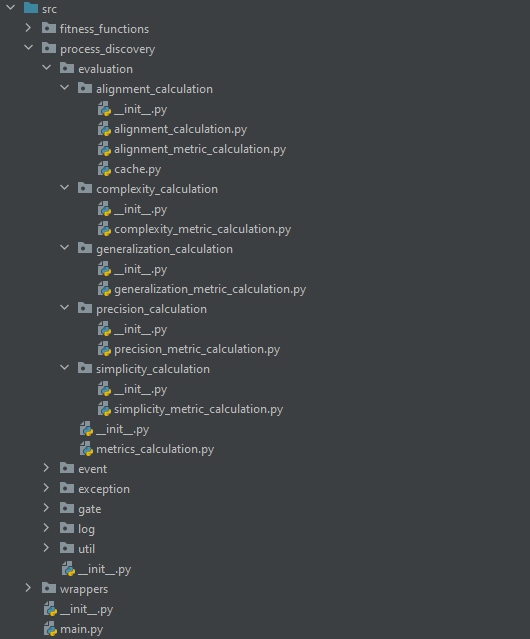
\includegraphics[scale=0.6]{Modules.png}}
	\caption{\label{fig:flow_chart}Podział na moduły}
\end{figure}

\subsection{Model}

Zdecydowano się na podział na dwie reprezentacje modelu procesu biznesowego wykorzystywane na różnym etapie procesowania. Wszystkie klasy implementują interfejs ComparableEvent pozwalający na ich porównywanie definiowanych przez nie obiektów. Aktywności są reprezentowane przez obiekty Event, które przechowują także informacje o ilości przejść w modelu przez dane zdarzenie, potrzebną do obliczenia generalizacji.   

Klasa Gate i klasy po niej dziedziczące są reprezentacją bliższą realnemu modelowi. 

\begin{figure}[h]
	\centering{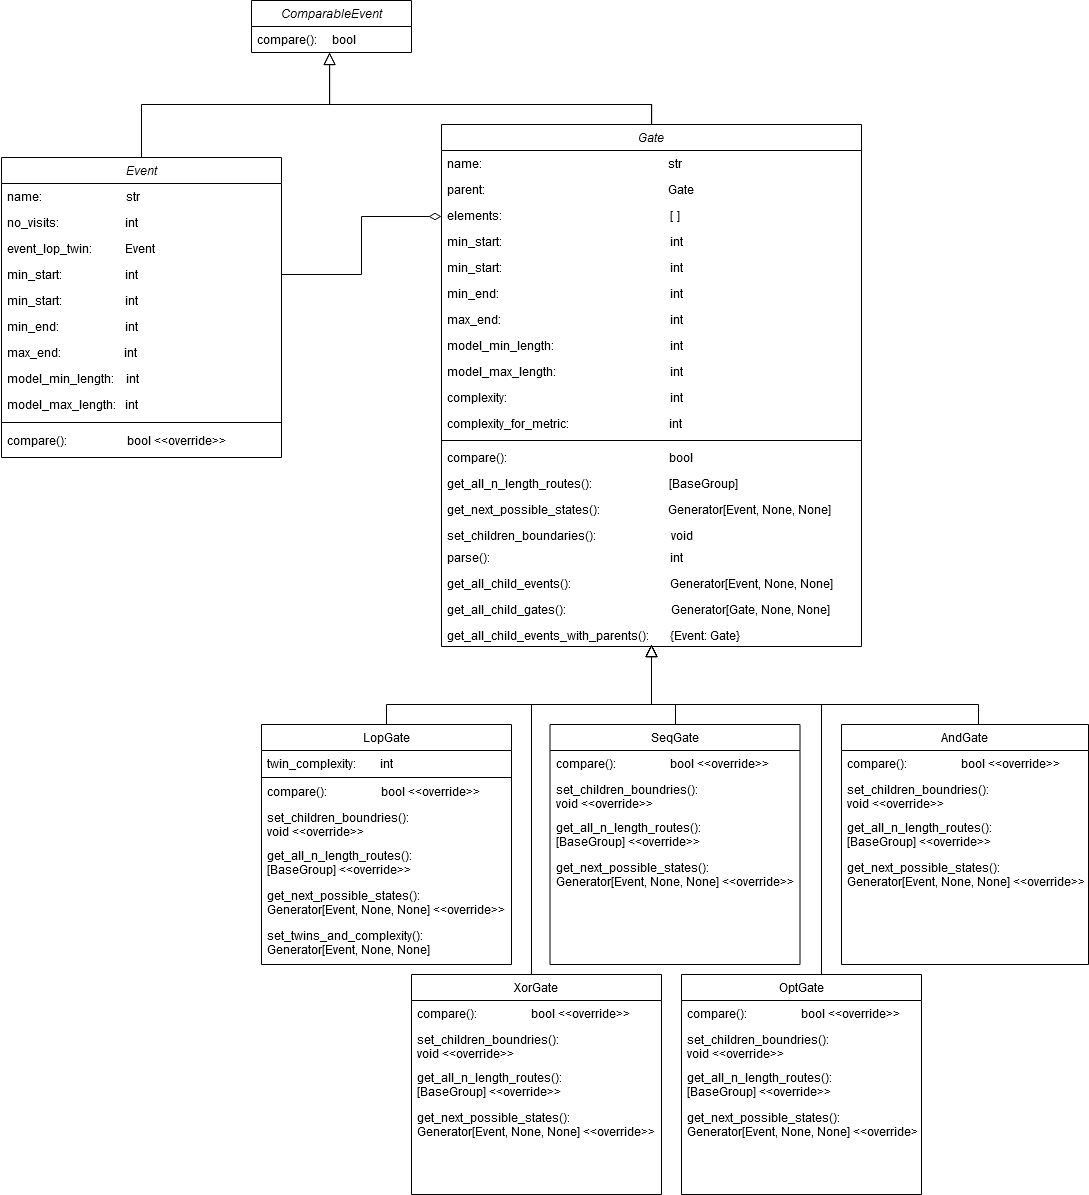
\includegraphics[scale=0.5]{GateUML.png}}
	\caption{\label{fig:subcaption_example}Gate UML}
\end{figure}

Model w formie ciągu znaków musi być zamieniony na formę, na której łatwiej będzie operować. Zakodowane zgodnie z zasadami gramatyki słowo zostaje sparsowane w metodzie parse() klasy Gate na obiekty klas po niej dziedziczących odpowiadające poszczególnym bramką logicznym. Obiekty posiadają wskaźnik na swojego rodzica, czyli bramkę - obiekt Gate, w której się znajduję oraz na bramki lub aktywności - obiekty Event, które zawierają. Przechowują też leniwie obliczaną informacja o złożoności. Najważniejsze metody, które klasy dziedziczące po Gate muszą nadpisać to:
\begin{itemize}
  \item[•] get$\_$next$\_$possible$\_$states() - zwraca jako generator możliwe kolejne aktywności, co jest potrzebne przy liczeniu precyzji.
  \item[•] get$\_$all$\_$n$\_$length$\_$routes() - zwraca możliwe ścieżki w modelu o danej długości jako tablicę obiektów BaseGroup, co jest potrzebne przy liczeniu odwzorowania
\end{itemize}

Obliczanie metryk dla klasy Gate byłoby utrudnione z uwagi na duża ilość bramek logicznych i konieczne jest przerobienie tych obiektów na formę pośrednią. Są nią obiekty klas dziedziczących po BaseGroup, które mają mieć formę ułatwiającą znajdowania dopasowania. Takie modularne podejście pozwala też na dodanie nowych bramek logiczny bez konieczności zmieniana metody obliczanie dopasowania, która jest najbardziej złożonym algorytmem występującym w programie. 

\begin{figure}[h]
	\centering{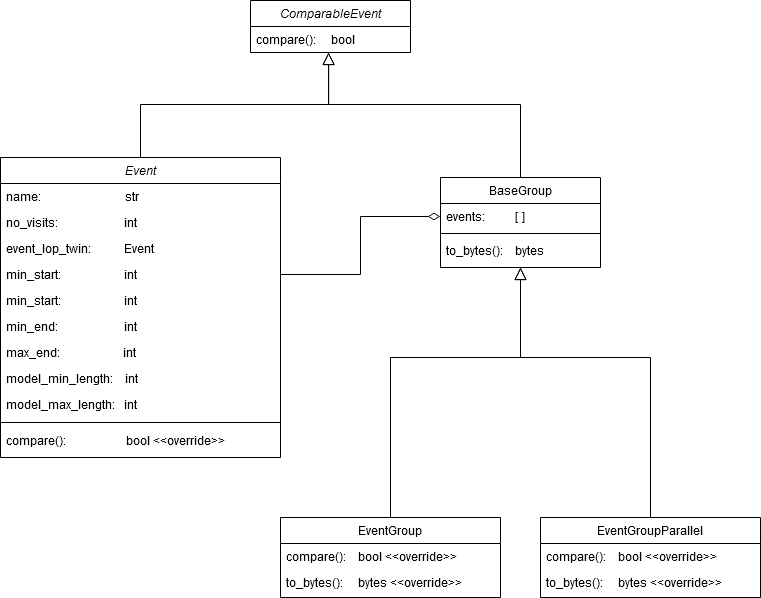
\includegraphics[scale=0.5]{EventUML.png}}
	\caption{\label{fig:subcaption_example}BaseGroup UML}
\end{figure}

W tej reprezentacji aktywności - obiekty Event są pogrupowane, jeśli występują razem, jednak zostawiamy tylko informacje potrzebne do liczenia dopasowania, czyli czy zdarzenia te mogą być wykonywane w dowolnej kolejność czy muszą być wykonywane kolejno po sobie. Dzięki temu stworzenie algorytmu do obliczania dopasowania jest łatwiejsze. Aktywności lub ich grupy są przechowywane jako lista. Jedyna metoda, która musi zostać nadpisana w klasach rozszerzających BaseGroup to to$\_$bytes() potrzebna przy cachowaniu. 

\section{Implementacja}

W tej części przedstawiono listingi z pseudokodem opartym na języku Python. Tam gdzie to konieczne pozostawiono słowa kluczowa oraz operatory tego języka.

\subsection{Ogólny schemat blokowy}


\begin{figure}[!ht]
	\centering{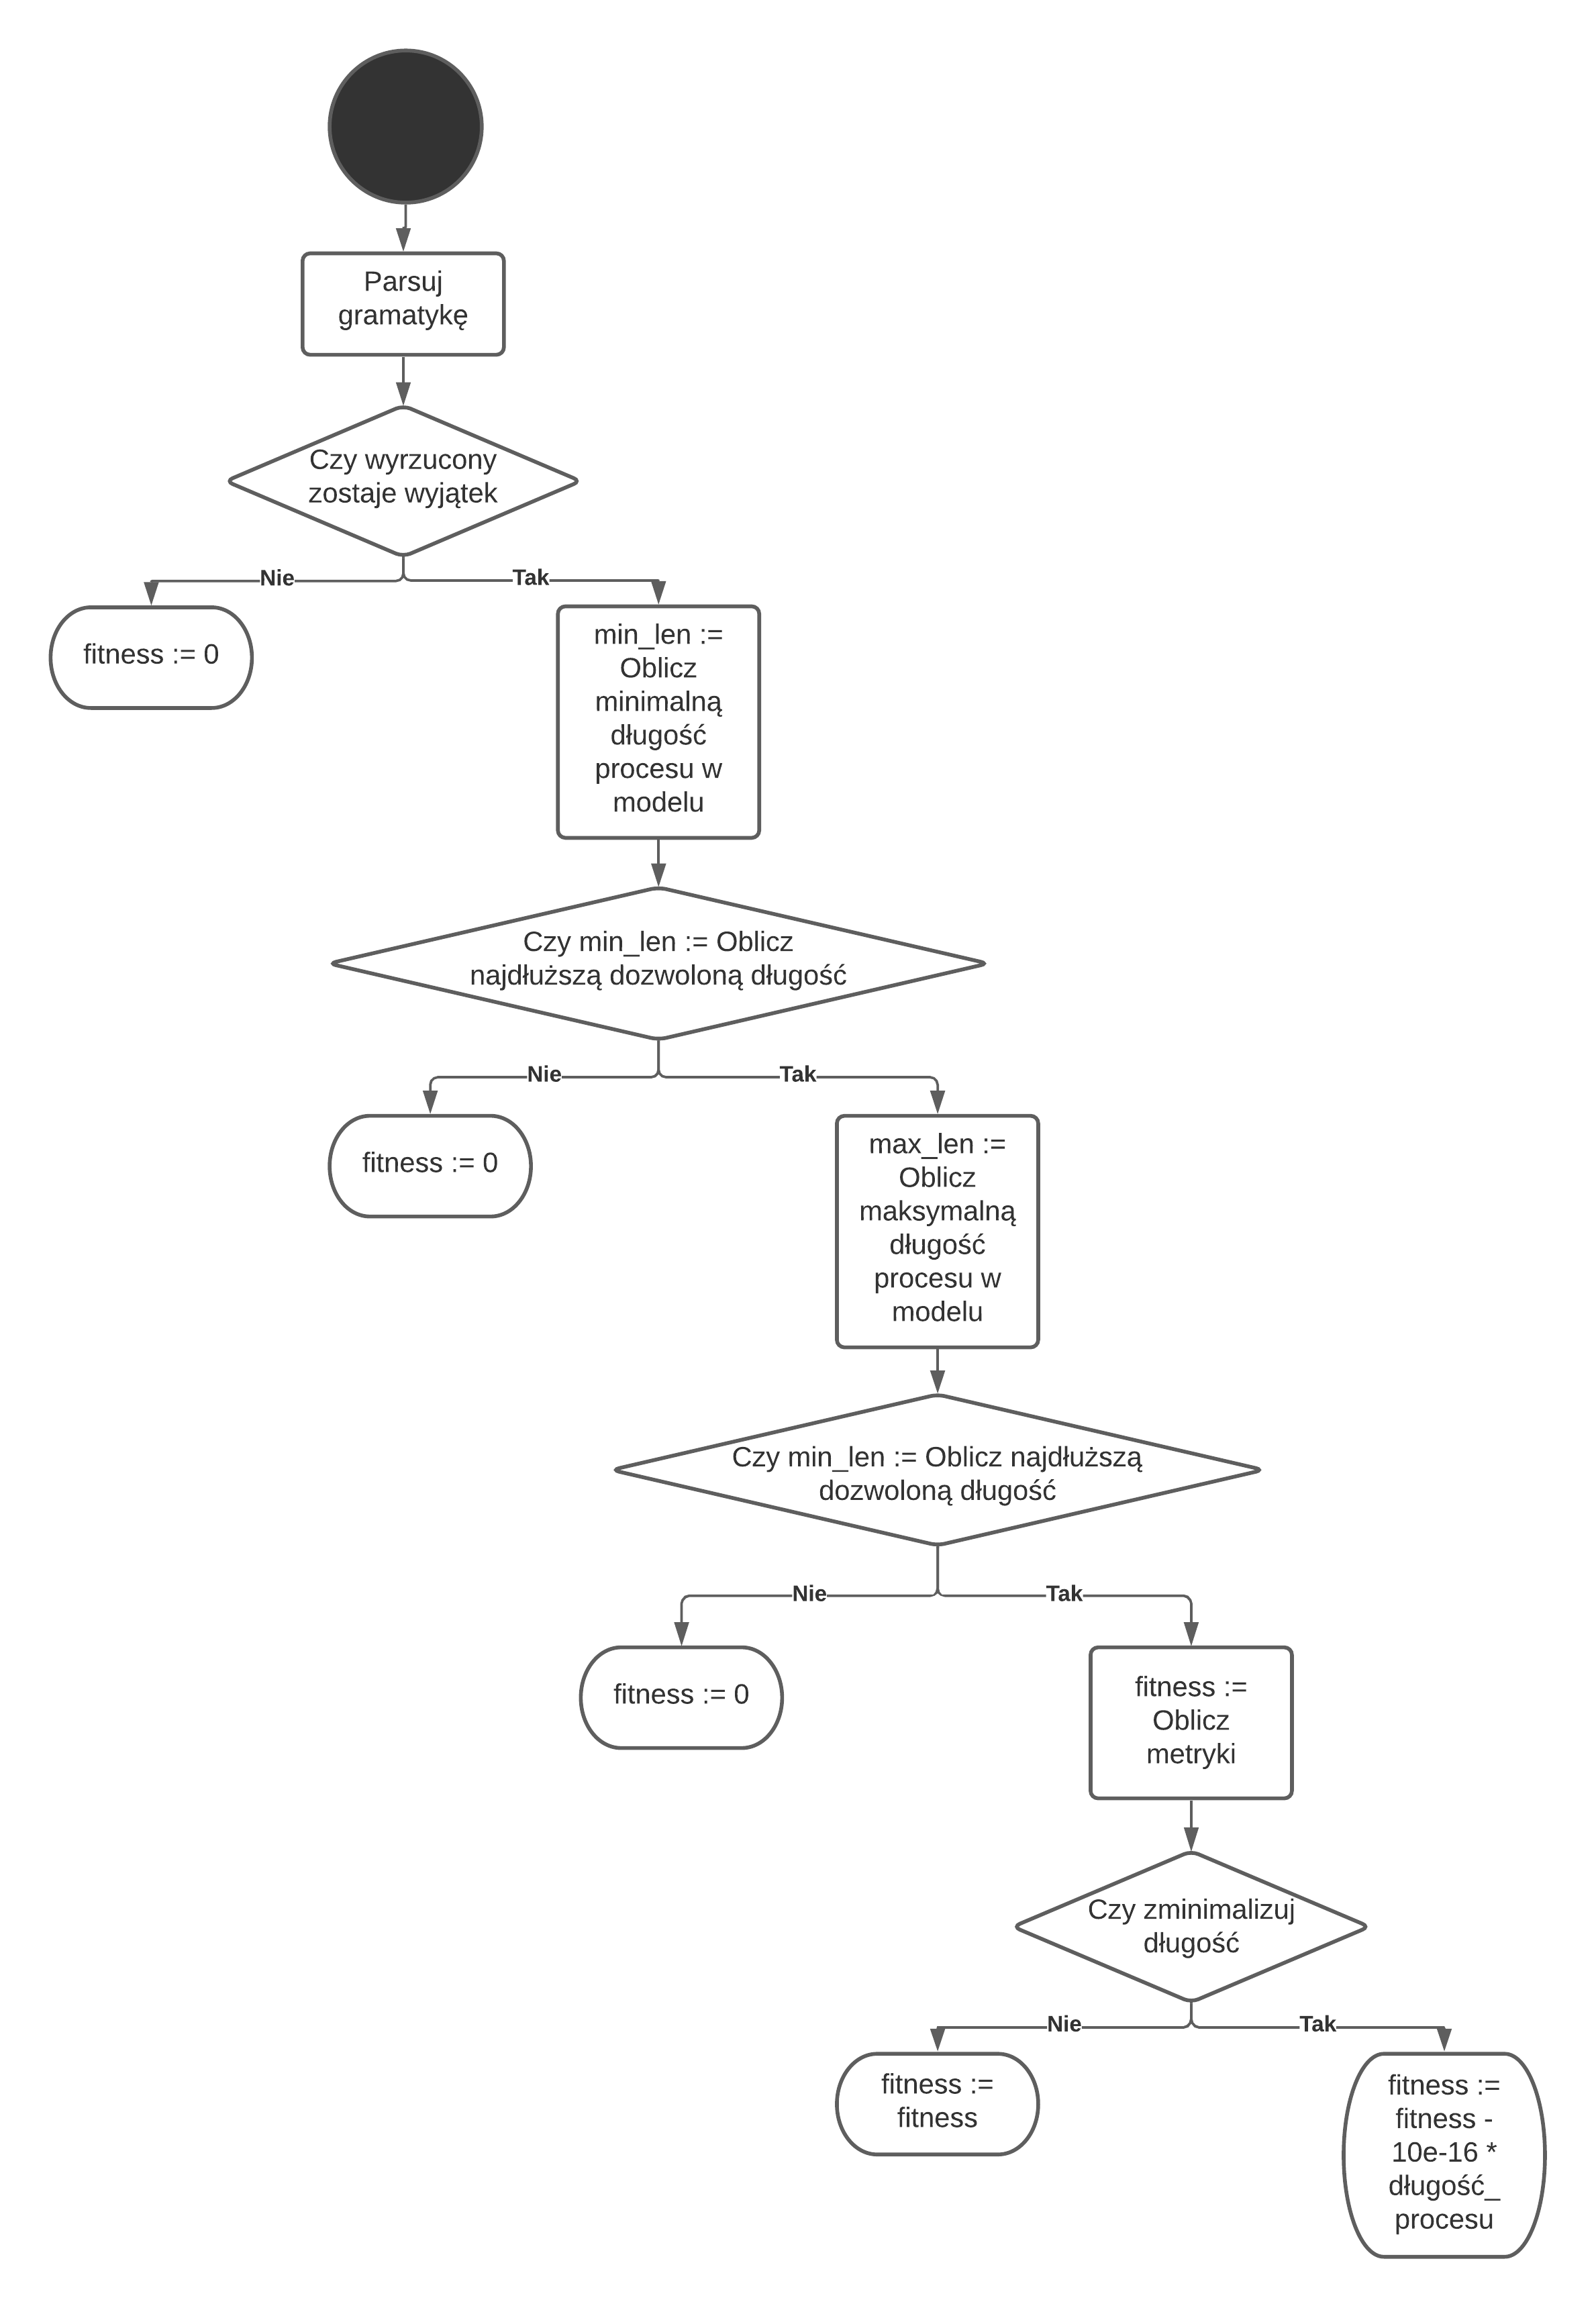
\includegraphics[scale=0.5]{OgolnySchematBlokowy.png}}
	\caption{\label{fig:flow_chart}Ogólny schemat blokowy}
\end{figure}

\subsection{Parsowanie gramatyki}
Parser pozwala na przetworzenie wyników uzyskanych na drodze ewolucji gramatycznej na postać, na której łatwiej będzie operować. Rezultaty uzyskane na drodze rewolucji gramatycznej w PonyGE2 są w formie tekstowej, z którą praca byłaby niewygodna, dlatego używamy parsera, żeby otrzymać wynik w postaci drzewa obiektów Gate, którego liśćmi będą obiekty Event.

Na tym etapie przeprowadzane są operacje takie jak:
Parsując korzystamy z faktu, że przy projektowaniu gramatyki wszystkie bramki logiczne zostały oznaczone 3 literowymi symbolami, a wszystkie zdarzenia otoczone nawiasami klamrowymi. Tworząc każdy obiekt Event dodajemy informację o liczbie dzieci tego obiektu, co przyda nam się przy obliczaniu metryki precyzja.
To na tym etapie odrzucamy też procesy, które mimo, że gramatyka pozwala na ich stworzenie inie moją sensu z punktu biznesowego, co pozwala na ograniczenie zasobów i nie przeliczanie dalszych rzeczy dla procesow, ktore sa bezwartosciowe. Odrzucamy procesy, ktore  

\lstset{caption=Parser gramatyki, captionpos=b}
\lstset{label=src:passive, frame=single}
\begin{lstlisting}[escapeinside=``]
def parsuj(wyrażenie: str) -> int:

   for i w zakresie długość_wyrażenia:
      if wyrażenie[i] == "{":
         zdarzenie := Event(wyrażenia[i + 1])
         dodaj zdarzenie do aktualnie parsowanej bramki 
         i += 2
      elif wyrażenie[i] == ")":
         return i+1
      elif i+4 < długość_wyrażenia:
          if wyrażenie[i:i + 3] == "seq" and (self.name == "seq" or self.name == "lop"):
             usuń_niepotrzebe_bramki
          else:
             if wyrażenie[i:i+2] == 'lo' and wyrażenie[i:i+3] != 'lop':  
                bramka := stwórz nową bramkę Gate typu zgodnego z wyrażeniem 
                i += 3
                przeparsowane_znaki = bramka.parsuj(wyrażenie[i+4:])
                if self.name == "seq" or self.name == "lop":
                   if int(wyrażenie[i+2]) <= długpść(gate.elementy):
                      for x in gate.elementy[int(wyrażenie[i+2]):]:
                         self.dodaj_element(x)
                dodaj zdarzenie do aktualnie parsowanej bramki 
                i += ilość_przeparsowanych_znaków
             else:
                bramka := stwórz nową bramkę Gate typu zgodnego z wyrażeniem 
                i += 3
                przeparsowane_znaki = bramka.parsuj(wyrażenie[i+4:])
                dodaj zdarzenie do aktualnie parsowanej bramki 
                i += ilość_przeparsowanych_znaków
       else:
          wyrzuć wyjątek
\end{lstlisting}

\subsection{Obliczanie metryk}
Mając już sparsowany model musimy obliczyć metryki. Najbardziej problematyczną metryką do obliczenia jest dopasowanie. Obliczanie dopasowanie można rozbić na następujące kroki:
\begin{itemize}
  \item[•] Znalezienie ścieżek o długości n w modelu.
  \item[•] Przerobienie ścieżek na postać zawierającą BaseGroup.
  \item[•] Obliczenie dopasowania.
\end{itemize}
Metryką, która nie wymaga obliczenia dopasowania jest prostota, dlatego możemy ją obliczyć wcześniej co przy niskim wyniku pozwala na wstępne odrzucenie części rezultatów bez konieczności kosztownego obliczania dopasowania. 
Pozostałe metryki wymagają obliczenia dopasowania i są obliczane dla najlepiej dopasowanej gramatyki.
Łatwo można zauważyć, że jeżeli zdarzenie znajduję się w logu, a nie znajduje się w modelu dopasowanie nie będzie dobre. Pozwala to odrzucić rezultaty, które nie przekraczają progu. 

\lstset{caption=Obliczanie metryk, captionpos=b}
\lstset{label=src:best_result, frame=single}
\begin{lstlisting}[escapeinside=``]
def oblicz_metryki(log_info, model, najkrótsza_dozwolona_długość, 
                   najdłuższa_dozwolona_długość, cache) -> int:
                   
   metryki['PROSTOTA'] := oblicz_metrykę_prostota(lista_zdarzeń_w_procesie), 
      unikalne_zdarzenia_w_logu)
   if metryki['PROSTOTA'] < 2/3:
      return 0
   stosunek_wspólnych_zdarzeń_w_logu_i_modelu := 
      oblicz_stosunek_wspólnych_zdarzeń_w_logu_i_modelu()		   
      if stosunek_wspólnych_zdarzeń_w_logu_i_modelu <
         MINIMALNY_STOSUNUK_WSPÓLNYCH_ZDARZEŃ_W_LOGU_I_MODELU:
      return stosunek_wspólnych_zdarzeń_w_logu_i_modelu/10
        
   idealnie_dopasowane_logi := pusty_słownik
   skumulowany_błąd := 0
    
   for proces w log:
      najlepszy_błąd_lokalny, najlepiej_dopasowana_ścieżka, najlepszy_process := 
      oblicz_metryki_dla_jednego_procesu(proces, model, minimalna_długość, 
      maksymalna_długość, cache)
      if jakikolwiek proces w najlepiej_dopasowanej_ścieżce nie znajduje się w modelu:
         value, best_aligned_process = obilcz_dopasowanie_bez_cache(best_event_group, 
            list(process), dict())
         best_local_error = calculate_alignment_metric(value, oblicz_długość(proces),
            oblicz_długość(best_event_group))
      if najlepszy_błąd_lokalny == 0:
         idealnie_dopasowane_logi.dodaj()
         [tuple(best_aligned_process)] = log_info.log[process]
      dodaj_wystąpienia(model_events_list, best_aligned_process, log_info.log[process])

   metryki := oblicz_metryki 
   najlepszy_wynik := oblicz_średnią_ważoną_metryk
   return najlepszy_wynik
\end{lstlisting}

\subsection{Obliczanie metryk dla jednego procesu}
Ważne jest, żeby jak najbardziej ograniczyć zbędne obliczenia.  W tym celu, co pozwoliło usprawnić cały proces

\lstset{caption=Obliczanie metryk dla jednego procesu, captionpos=b}
\lstset{label=src:best_result, frame=single}
\begin{lstlisting}
def oblicz_metryki_dla_jednego_procesu(proces, model, najkrótsza_dozwolona_długość, 
				               najdłuższa_dozwolona_długość, cache):
   dłogość_procesu := oblicz_długość(proces)
   n := dłogość_procesu
   i := 1
   minimalny_błąd_dopasowania := -(dłogość_procesu + model.model_min_length)
   while not (dolny_limit_osiągnięty and górny_limit_osiągnięty):
      if n >= min(oblicz_maksymalną_dozwoloną_długość(dłogość_procesu), 
                  dłogość_procesu - minimalny_błąd_dopasowania):
         górny_limit_osiągnięty := True
         n += (-i if i % 2 == 1 else i); i += 1
         continue
      if n <= max(oblicz_minimalną_dozwoloną_długość(dłogość_procesu), 
                  dłogość_procesu + minimalny_błąd_dopasowania):
         dolny_limit_osiągnięty := True
         n += (-i if i % 2 == 1 else i); i += 1
         continue
      if najkrótsza_dozwolona_długość <= n <= najdłuższa_dozwolona_długość:
         ustaw_najwcześniejsze_i_najpóźniejsze_wystąpienie_zdarzenia(model, n)
         ścieżki = model.znajdź_wszystkie_ścieżki_długości_n(n, proces)
         if ścieżki istnieją:
            for ścieżka in ścieżki:
               procent_wspólnych_zdarzeń := oblicz_procent_wspólnych_zdarzeń_
                  w_modelu_i_logu(ścieżka, proces)
               if procent_wspólnych_zdarzeń >= 1 - TOLERANCJA:
                  dodaj sćiezkę do lista_ścieżek_do_obliczenia
            posortowane_ścieżki := posortuj lista_ścieżek_do_obliczenia
            for ścieżka in posortowane_ścieżki:
               if procent_wspólnych_zdarzeń <= 1 + minimalny_błąd_dopasowania /
                  długość_procesu:
                  break
               błąd_dopasowania, najlepsze_dopasowane_zdarzenia, jest_z_cache :=
                  oblicz_najlepsze_dopasowanie_z_cache(ścieżka, proces, cache)
               if błąd_dopasowania > minimalny_błąd_dopasowania:
                  minimalny_błąd_dopasowania := błąd_dopasowania
                  najlepsze_dopasowane_zdarzenia := dopasowane_zdarzenia
                  najlepsza_ścieżka := scieżka
                  jest_najlepszy_z_cache := jest_z_cache
               if błąd_dopasowania == 0:
                  return minimalny_błąd_dopasowania, najlepsze_dopasowane_
                         zdarzenia, najlepsza_ścieżka, jest_najlepszy_z_cache
      n += (-i if i % 2 == 1 else i); i += 1
   return minimalny_błąd_dopasowania, najlepsze_dopasowane_zdarzenia, 
          najlepsza_ścieżka, jest_najlepszy_z_cache
\end{lstlisting}

\subsection{Wyszukiwanie w modelu procesów o określonej długości}

Łatwiejszym jest znalezienie wszystkich ścieżek o określonej długości. Najprawdopodobniejsze jest, ze najlepiej dopasowana ścieżka będzie miała długość jak wejście w logu dlatego zaczyna od tej długości. 
Algorytm rekurencyjny. Implementacja różni się w zależności od przeszukiwanej bramki logicznej. Poniżej zaprezentowano przykład dla bramki.  
\lstset{caption=Wyszukiwanie procesów o długości n, captionpos=b}
\lstset{label=src:get_n_length, frame=single}
\begin{lstlisting}[escapeinside=``]
def znajdź_wszystkie_ścieżki_długości_n(n, proces) -> []:
    if n == 0:
        return []
    if self.model_max_length < n or n < self.model_min_length:
        return None

    min_lengths = self.get_children_min_length()
    max_lengths = self.get_children_max_length()
    global_list = []

    for elem in self.elements:
        local_list = []
        if isinstance(elem, Event):
            local_list.append(elem)
            min_lengths.pop(0)
            max_lengths.pop(0)
        else:
            lower_limit, upper_limit = self.get_goal_length_range(n, global_list, min_lengths, max_lengths)
            for i in range(lower_limit, upper_limit + 1):
                try:
                    child_all_n_length_routes = elem.get_all_n_length_routes(i, process)
                except ValueError:
                    return None
                if child_all_n_length_routes is not None:
                    local_list.append(child_all_n_length_routes)

        if local_list:
            global_list.append(local_list)

    result = []
    if global_list:
        for elem in flatten_values(global_list):
            if self.check_length(n, elem):
                if n == 1:
                    # because always 1 elem list
                    result.append(elem[0])
                else:
                    self.check_valid_for_get_n_length(elem)
                    result.append(EventGroupParallel(elem))
    if result:
        return result
    else:
        return None
\end{lstlisting}

\subsection{Obliczanie dopasowania}
Pomysł zaczerpnięty z algorytmu Needlessmann-Wunsch \cite{ea252fd3937a4a309a5e07e61e5531a7}, który jest uogólnieniem odległości Levenshteina. Tworzymy macierz o wymiarach długość modelu i długość logu, w której obliczać będziemy rozwiązania. Rozwinięty o możliwość przeszukiwania modelu rekurencyjnie oraz o możliwość podawania listy równoległych zdarzeń. 
\lstset{caption=Obliczanie dopasowania, captionpos=b}
\lstset{label=src:alignment_calculation, frame=single}
\begin{lstlisting}[escapeinside=``]
def oblicz_dopasowanie(model, log):
    błąd := {'DOPASOWANIE': 0, 'BRAK_DOPASOWANIA': -2, 'PRZERWA': -1}
    m = długość(model) + 1  # Macierz rozwiązań ilość wierszy.
    n = długość(log) + 1  # Macierz rozwiązań ilość kolumn.
    najlepiej_dopasowana_ścieżka := [None] * m
    macierz_rozwiazań := Zainicjalizuj macierz zerami
    # Wypelnij osie macierzy właściwymi wartościami
    for j in range(n):
        macierz_rozwiązań[0][j] := błąd['PRZERWA'] * j

    for i in range(1, m):
        if should_go_recurrent(model[i-1]):
            macierz_rozwiązań[i], najlepiej_dopasowana_ścieżka_podmodelu[i] := 
            dopasowanie_rekurencyjne(macierz_rozwiazań[i - 1], model[i - 1],
                                     [x for x in odwrócone_substringi(log)], i)
        elif długość(model[i-1]) > 1:
            macierz_rozwiązań[i], najlepiej_dopasowana_ścieżka_podmodelu[i] := 
            dopasowanie_równoległe(macierz_rozwiazan[i - 1], model[i - 1],
                                   [x for x in odwrócone_substringi(log)], kara, i)
        else:
            macierz_rozwiazań[i][0] := macierz_rozwiązań[i-1][0] + kara['PRZERWA']
            dopasowanie(macierz_rozwiazań, model[i - 1], log, kara, i, n)

    ścieżka := znajdź_ściezkę(macierz_rozwiązań, błąd['PRZERWA'], model, 
    log, najlepiej_dopasowana_ścieżka_podmodelu)

    return macierz_rozwiązań[m-1], najlepiej_dopasowana_ścieżka
\end{lstlisting}

\subsection{Znajdowanie ścieżki w modelu}
Potrzebne do obliczenia precyzji oraz generalizacji. Z wzgledu na zmiany
\lstset{caption=Znajdowanie ścieżki w modelu, captionpos=b}
\lstset{label=src:traceback, frame=single}
\begin{lstlisting}[escapeinside=``]
def znajdź_sciezkę(macierz_rozwiązań, model, log, rozwiązania_podmodeli):
    sciezka = []
    while i != 0:
        długość_grupy_zdarzeń = długość(model[i - 1])
        if model_results_local[i] is not None:
            znaleziono_dopasowanie := False
            if macierz_rozwiązań[i][j] == macierz_rozwiązań[i - 1][j] + długość_grupy_zdarzeń * błąd['PRZERWA']:
                [model_result.append(None) for _ in range(długość_grupy_zdarzeń)]
                macierz_rozwiązań[i][j] := 0
                i -= 1
            else:
                for k in range(j):
                    zdarzenia := get_not_none(model_results_local[i][k]
                    [długość(model_results_local[i][k]) - (j-k)], log)
                    if macierz_rozwiązań[i][j] == macierz_rozwiązań[i - 1][k] + 
                    	(długość_grupy_zdarzeń + (j-k) - 2 * długość(processes)) * błąd['PRZERWA']:
                        [model_result.append(x) for x in processes]
                        for x in processes:
                            log = log.replace(x.name, "", 1)
                        [model_result.append(None) 
                         for _ in range(długość_grupy_zdarzeń - len(processes))]
                        macierz_rozwiązań[i][j] = 0
                        i -= 1; j = k
                        znaleziono_dopasowanie = True
                        break
                if not znaleziono_dopasowanie:
                    if macierz_rozwiązań[i][j] == macierz_rozwiązań[i][j - 1] + błąd['PRZERWA']:
                        macierz_rozwiązań[i][j] = 0
                        j -= 1
        else:
            if macierz_rozwiązań[i][j] == macierz_rozwiązań[i - 1][j] + kara:
                model_result.append(None)
                macierz_rozwiązań[i][j] := 0
                i -= 1
            elif macierz_rozwiązań[i][j] == macierz_rozwiązań[i][j - 1] + kara:
                macierz_rozwiązań[i][j] := 0
                j -= 1
            elif macierz_rozwiązań[i][j] == macierz_rozwiązań[i - 1][j - 1]:
                model_result.append(model[i-1])
                log = log.replace(model[i-1].name, "", 1)
                macierz_rozwiązań[i][j] := 0
                i -= 1; j -= 1
    return sciezka
\end{lstlisting}

\subsection{Pozostałe wnioski dotyczące implementacji}
Cache

W sytuacji kiedy wiele obliczeń się powtarza można znacząca przyspieszyć czas działania aplikacji poprzez zastosowanie cachowania. W przypadku naszego algorytmu można zauważyć dwa miejsca, w których często dochodzi to powtórzeń:
Poprzednio obliczone rozwiązanie może się powtórzyć. W tym wypadku możemy skorzystać z cache genotypów, dostarczane przez bibliotekę PonyGE2.
Podczas obliczania dopasowania, które jest najbardziej kosztownym obliczeniem. Ponadto z uwagi na duża ilość obliczeń, żeby ograniczyć rozmiar cache zaimplementowano cachowanie LRU.
\section{Wybór parametrów algorytmu}
Wybór parametrów algorytmu ma ogromny wpływ na jakość i szybkość znalezienia rozwiązania. Jest kilka zasad, którymi należy się kierować przy tym wyborze właśnie. Ilość parametrów wymagana przez ponyGE2 jest duża, dodatkowo tworząc mimo, że starano się ograniczyć możliwość konfiguracji, która nie daje dużo korzyści do minimum tworząc aplikacje dodano kilka innych niezbędnych parametrów. Z tego powodu, poniżej przedstawiono i krótko omówiono niezbędne do działania aplikacji parametry.

Włącza cache: \newline
\textit{CACHE:                         True} \newline
\textit{CODON\_SIZE:                   100000} \newline
Ilość wątków procesora:
\textit{CORES:                         4} \newline
\textit{CROSSOVER:                     subtree} \newline
\textit{CROSSOVER\_PROBABILITY:         0.75} \newline
\textit{DEBUG:                         False} \newline
\textit{ELITE\_SIZE:                   30} \newline
\textit{GENERATIONS:                   100000} \newline
\textit{MAX\_GENOME\_LENGTH:           500} \newline
\textit{GRAMMAR\_FILE:                  process-subtree.bnf} \newline
\textit{INITIALISATION:                 PI\_grow} \newline
\textbf{INVALID\_SELECTION:              False} \newline
\textbf{LOOKUP\_FITNESS:                 True} \newline
\textbf{MAX\_INIT\_TREE\_DEPTH:            13} \newline
\textbf{MAX\_TREE\_DEPTH:                 21} \newline
\textbf{MULTICORE:                      True} \newline
\textbf{MULTI\_OBJECTIVE:                False} \newline
\textbf{MUTATION:                       subtree} \newline
\textbf{MUTATION\_EVENTS:                1} \newline
\textbf{POPULATION\_SIZE:                500} \newline
\textbf{FITNESS\_FUNCTION:               process\_fitness} \newline
\textbf{REPLACEMENT:                    generational} \newline
\textbf{SAVE\_STATE\_STEP:                10} \newline
\textbf{SELECTION:                      tournament} \newline
\textbf{TOURNAMENT\_SIZE:                16} \newline
\textbf{VERBOSE:                        True} \newline
\textbf{MAX\_WRAPS:                      3} \newline
\textbf{ALIGNMENT\_CACHE\_SIZE:           32*1024} \newline
\textbf{DATASET:                        discovered-processes.csv} \newline
\textbf{MAX\_ALLOWED\_COMPLEXITY\_FACTOR:  300} \newline
\textbf{MINIMIZE\_SOLUTION\_LENGTH:       True} \newline
\textbf{RESULT\_TOLERANCE\_PERCENT:       5} \newline
\textbf{TIMEOUT:                        5} \newline

Rekomendowane wagi poszczególnych metryk: \newline
\textbf{WEIGHT\_ALIGNMENT:              8} \newline
\textbf{WEIGHT\_COMPLEXITY:              2} \newline
\textbf{WEIGHT\_GENERALIZATION:          2} \newline
\textbf{WEIGHT\_PRECISION:               2} \newline
\textbf{WEIGHT\_SIMPLICITY:              2} \newline
